The GPS and SQISign protocols we describe in this section work with the full supersingular  isogeny graph (unlike the CSIDH-based protocols of Section~\ref{sec:CSIDH} which only consider curves defined over $\mathbb{F}_p$), and use the quaternion algorithms described in Section~\ref{sec:KLPT} to design a GMW-like protocol which does not rely on a SIDH diagram. 
The GPS protocol provides steps towards a general solution to proving the relation $\R[isog]$.
In particular, the GPS protocol achieves statistical ZK, and no auxiliary points or other information are needed to obtain zero-knowledge.



\subsection{GPS sigma protocol} \label{sec:GPSproof}



%This section explains how to take the naive protocol from Section~\ref{sec:simple} and make it secure. The key idea is a method to ``re-randomise'' $\rho = \psi \circ \phi$, so that the response to the challenge is a uniformly sampled isogeny from $E_0$ to $E_2$.
%This conjecturally gives statistical ZK. \CP{why ``conjecturally''?}

The GPS protocol, due to Galbraith, Petit and Silva~\cite{GPS20},  heavily uses the ideas of Section~\ref{sec:KLPT}. In particular, we assume that $E_0$ is a special supersingular curve such as $y^2 = x^3 + x$.
We wish to prove knowledge of an isogeny $\phi : E_0 \to E_1$, and will use properties of $\End(E_0)$.
So our protocol proves $\R[isog]$ for any field, but in the special case where $E_0$ is a curve with known endomorphism ring.

To prove knowledge of an isogeny between two ``arbitrary'' curves $E'$ and $E''$ one can apply this protocol if one knows an isogeny from $E_0$ to $E'$ (and hence one can construct an isogeny from $E_0$ to $E''$).
However, if $E'$ and $E''$ are curves whose endomorphism ring is not known to the prover then the methods of this section cannot be applied.

The sigma protocol is as follows.
First, fix parameters $B$, $N_1$, $N_2$ such that $N_k =\prod_i\ell_{k,i}^{e_{k,i}}$, where $\ell_{k,i}^{e_{k,i}}<B$, $\gcd(N_1,N_2)=1$, $\log(N_2) > \tfrac{7}{2} \log(p)$, and for each $k \in \{1,2\}$
\[
  \prod_i\left(\frac{2\sqrt{\ell_{k,i}}}{\ell_{k,i}+1}\right)^{e_{k,i}}<(p^{1+\epsilon})^{-1}. 
\]
This last formula is needed for uniform mixing of random walks in the isogeny graph.
We let $I$ be the left $\OO_0$-ideal corresponding to the secret isogeny $\phi : E_0 \to E_1$.

To construct the commitment $\com$, perform a random isogeny walk of degree $N_1$ from the curve $E_1$ to a curve $E_2$ and set $\com = j(E_2)$.
The isogeny $\psi : E_1 \to E_2$ can be represented in many ways (e.g., kernel points of order $\ell_i^{e_i}$ or a sequence of $j$-invariants).
Let $J$ be the left-$\End(E_1)$-ideal corresponding to $\psi$.
Let the challenge be $\chall \in \{0,1\}$.
When $\chall=0$ respond with $\psi$.
When $\chall=1$ the KLPT algorithm is needed. We compute the ideal $IJ$, which corresponds to $\psi \circ \phi$.
Then run KLPT to get an equivalent $\OO_0$-ideal $J'$ of norm $N_2$. The response is the isogeny $\psi' : E_0 \to E_2$ corresponding to $J'$.
The verifier checks that the response is an isogeny from $E_{1-\chall}$ to $E_2$.
The protocol is repeated until the verifier is convinced.

Special soundness of the protocol is easy to prove. Given valid responses $\psi'$ and $\rho$ to the challenges 0 and 1 for the same commitment, the extractor can compute an isogeny $\rho\hat\psi'$ from $E_0$ to $E_1$. Note that this isogeny is a priori not the same one used by the prover  to create the responses, but this is irrelevant to special soundness\footnote{Additionally, both isogenies can in fact be mapped to the same ``canonical'' one (for example, using LLL to compute a minimal norm ideal in the ideal class, followed if needed by some deterministic version of KLPT to get a powersmooth norm ideal).}.


The three key requirements for this to be zero-knowledge and practical are that:
\begin{enumerate}
    \item $E_2$ is close to uniformly distributed in the isogeny graph.
    \item The isogeny $\psi'$ is independent of $\phi$.
    \item The isogenies $\psi$ and $\psi'$ in the response have a compact representation and can be computed efficiently.
\end{enumerate}
The first two properties are needed for zero-knowledge. 
The simulator, who knows the challenge but who does not know $\phi$ or $I$, will behave as in the honest protocol for the case $\chall=0$, but when $\chall=1$ will take a random isogeny from $E_0$ to $E_2$ and then run KLPT to get an ideal $J'$ as in the real protocol. 
It is necessary that the curves $E_2$ generated by the simulator when $\chall=1$ are distributed close to identically as in the original protocol. This is the purpose of the first requirement.
It is also necessary that the isogenies $\psi'$ are distributed identically in both cases.
We refer to~\cite{GPS20} for the details.


As the protocol uses one-bit challenges, it must be repeated $\lambda$ times to obtain a scheme with $2^{-\lambda}$ soundness error.
The protocol can be made non-interactive and used as a signature scheme by the Fiat-Shamir transform. While polynomial time in theory, the resulting signature scheme is considered impractical.
%, and it has never been implemented.


%This is still using single bit challenges.
%In some cases (depending on the witness $\phi$) we might be able to apply the ideas of SQI-Sign. \CP{I don't get the last sentence}




\subsection{SQISign \label{sec:SQIsign}}

A key source of inefficiency in GPS signatures (and other signatures based on isogenies) is the need to repeat the zero-knowledge protocol multiple times to reduce the soundness error. This comes from the fact that the protocol has single bit challenges.


To increase the challenge space, the SQISign protocol by De Feo, Kohel, Leroux, Petit and Wesolowski modifies the basic GMW-based protocol as follows. Given a secret isogeny $\phi:E_0\rightarrow E_1$, the prover first computes a random isogeny $\psi:E_0\rightarrow E_2$ and commits to $E_2$. Then instead of challenging the prover with a single bit, the verifier computes and sends a third random isogeny $\varphi:E_2\rightarrow E_3$, sends it to the prover, and challenges the prover to compute an isogeny $\sigma:E_1\rightarrow E_3$ (see Figure~\ref{fig:sqisign}).

\begin{figure}[h!]
    
  
\begin{center}
   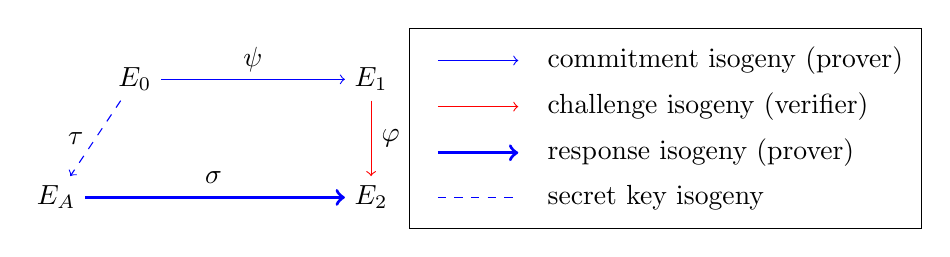
\begin{tikzpicture}
    \node (E0) at (1,2.5) {$E_0$};
    \node (E1) at (4,2.5) {$E_1$};
    \node (E2) at (4,1) {$E_2$};
    \node (EA) at (0,1) {$E_A$};
    \node (A) at (0.25,1.75) {$\tau$};
    \node (B) at (2.5,2.75) {$\psi$};
    \node (A) at (4.25,1.75) {$\varphi$};
    \node (B) at (2,1.25) {$\sigma$};
    % \draw [->] (E) -- (E1);
    \draw [blue,very thick] [->] (EA) -- (E2);
    \draw [red] [->] (E1) to (E2);
    \draw [blue,dashed] [->] (E0) to (EA);
    \draw [blue] [->] (E0) to (E1);
    \matrix [draw, right] at (current bounding box.east) {
\node[] (l1) {}; \node (l2) [right of = l1, node distance=0.5in,label=right: commitment isogeny (prover)] {}; \draw [blue] [->] (l1) -- (l2); \\
\node[] (l3) {}; \node (l4) [right of = l3, node distance=0.5in,label=right:challenge isogeny (verifier)] {}; \draw [red] [->] (l3) -- (l4); \\
\node[] (l1) {}; \node (l2) [right of = l1, node distance=0.5in,label=right: response isogeny (prover)] {}; \draw [blue,very thick] [->] (l1) -- (l2); \\
\node[] (l1) {}; \node (l2) [right of = l1, node distance=0.5in,label=right: secret key isogeny] {}; \draw  [dashed,blue] [-] (l1) -- (l2); \\
};
\end{tikzpicture}
\end{center} \caption{A picture of SQIsign's identification protocol~\cite{DFKLPW20}}   \label{fig:sqisign} \end{figure}

%\WB{reviewer says: "a commutative diagram to accompany the second paragraph of section 6.2 would be a worthy addition imo"}

A naive version of this protocol is not secure: A dishonest prover could compute the commitment by computing a random isogeny $\psi'$ from $E_1$. Call $E_2$ the image curve. Since the verifier sends an isogeny $\varphi$ the prover can respond with $\varphi \circ \psi' : E_1 \to E_3$.
The way to prevent this is for the verifier to check that $\hat{\varphi} \circ \sigma$ has cyclic kernel; we refer to~\cite{DFKLPW20} for the details.
The protocol also imposes conditions on the isogeny $\phi:E_0\rightarrow E_1$, namely that $E_0$ has known endomorphism ring and that $\phi$ has ``medium'' prime degree.
Finally, the protocol is only computationally ZK based on an ad hoc assumption.
Hence SQISign is currently far from a general solution to the relation $\R[isog]$.

Special soundness relies on the problem of computing an endomorphism of $E_1$, a problem equivalent to computing an isogeny between two random supersingular  curves~\cite{GPS20,Reductions18,Wes22}.


%
Indeed, given two valid responses to two challenges for the same commitment, an extractor can compose both challenges and responses in an appropriate way  to compute an endomorphism of $E_1$ (see~\cite{DFKLPW20}).\footnote{A similar approach in the case of graph isomorphism would provide the extractor with an automorphism of one graph. This does not immediately solve the graph isomorphism problem.}
%\CP{but  can maybe be used to accelerate Babai's algorithm?}}.

The astute reader will have noticed that computing $\sigma$ now requires to re-randomize an isogeny between two random supersingular curves, whereas the tools described in Section~\ref{sec:KLPT} assumed one of the curves was ``special'', i.e. with known and very special endomorphism ring. One can trivially generalize these tools to the general case (in fact this was already done in~\cite{KLPT}), but in a way that, used in the above signature scheme, will always leak the secret (the isogeny $\sigma$ will always go through the curve $E_0$). 
%
The key contribution in~\cite{DFKLPW20} is a new generalization of the KLPT algorithm which conjecturally avoids this problem. 

SQISign signatures are an order of magnitude smaller than all other post-quantum isogeny-based signature schemes in the signature-plus-public-key metric. Key generation and verification time are reasonable (at 0.6s and 50ms respectively) but signing takes 2.5s, mostly because of the conversions between isogenies and ideals (which are polynomial time but slow in practice).
%
An improved version of the protocol obtained a two-fold speedup on signing time~\cite{SQIsign2.0}.
%
This however remains too slow for many applications. 

Further work should aim at improving the signing time, but also to address some outstanding security concerns:
\begin{itemize}
    \item SQISign is not known to be secure in the quantum oracle model. This is because the sigma protocol does not have any of the properties that allow to prove the security of Fiat-Shamir signatures in this model~\cite{KLS18}. Possible solutions include switching to the Unruh transform~\cite{Unruh15} (at some efficiency cost) or developing an ad hoc proof.
    \item The SQISign security proof does not provide an extractor that outputs an isogeny from $E_0$ to $E_1$. So it is not technically a proof of knowledge for $\R[isog]$. 
    However, the extractor does return a ``random'' endomorphism on $E_1$.
    
    Heuristically, $O(1)$ independent endomorphisms should generate the whole endomorphism ring, and one can build~\cite{EHLMP20} a $k$-special sound extractor that computes the whole endomorphism ring (for $k=O(1)$). Proving this formally remains an open problem.
    Once $\End(E_1)$ is known then an isogeny from $E_0$ to $E_1$ can be computed~\cite{Wes22}.
    %
    \item The security definition for computational honest verifier zero-knowledge in Definition~\ref{def:sigmaprot} allows the distinguisher to be provided with a witness, but the arguments for the computational honest verifier zero-knowledge property in~\cite{DFKLPW20} do not apply in this case. Indeed with a witness one can easily distinguish between the response isogeny and a random isogeny of the same degree between the same two curves (as a quick study of~\cite[Figure 3]{DFKLPW20} shows). One approach to solve this problem could be randomize the output of the \emph{EquivalentPrimeIdeal} and/or the particular secret isogeny $\tau$ used in the generalized KLPT algorithm~\cite{DFKLPW20}. However, both approaches will increase the norm of the ideal output by this algorithm hence further slow down signature generation. We also leave the security analysis of these approaches to further work.
\end{itemize}






